\chapter{Image Compression}

Image compression is a technique used to reduce the size of image files. For instance, a image encoded using $8$ bits for each of the RGB channels (i.e., $24$ bits per pixel) in a $3200\times 2000$ pixel image would require $\unit[18.31]{MB}$ of storage. Applying different types of compression can significantly reduce the file size, making it easier to store and transmit images. There are two main types of image compression: lossless and lossy. Lossless compression allows the original image to be perfectly reconstructed from the compressed data, while lossy compression results in some loss of quality but can achieve much higher compression ratios.

\section{Lossless Compression}

As already mentioned, lossless compression allows the original image to be perfectly reconstructed from the compressed data, resulting in no loss of quality. We will first cover some of the most common lossless compression techniques, and then the main lossless image formats.
\begin{observacion}
    Even though compression techniques are designed to reduce file size, there is no technique that can guarantee that all files will be compressed. If that were the case, we could compress a file repeatedly until we get a file of size zero, which is not possible. In practice, most compression techniques will be able to compress most files, but there will always be some files that cannot be compressed or that may even increase in size after compression.
\end{observacion}

\subsection{Run Length Encoding}

The Run Length Encoding (RLE) is a simple lossless compression technique that works by replacing sequences of repeated characters with a single character and a count of how many times it is repeated. For example:
\begin{center}
    \texttt{AAAABBBCCDAA} $\rightarrow$ \texttt{4A3B2C1D2A}
\end{center}

There are always some conventions that should be previously established to avoid ambiguity. For instance, when a character is repeated only once, we can choose to omit the count and just write the character itself. In that case, the previous example would be encoded as:
\begin{center}
    \texttt{AAAABBBCCDAA} $\rightarrow$ \texttt{4A3B2CD2A}
\end{center}

However, some problems may arise:
\begin{itemize}
    \item If numbers also appear in the original string, we need to establish a convention to distinguish between counts and characters. A control char ($X$ for instance) can be used to indicate that the following character is a count. For example:
\begin{center}
    \texttt{121211111111122222212111} $\rightarrow$ \texttt{1212X91X6212X31}
\end{center}
    This still has some problems, as the count could be greater than $9$, which would require more than one character to represent it. In that case, we can use a different control char (e.g., $Y$) to indicate the final of the count.

    \item If the original string contains the control char itself, we need to establish a convention to escape it. For example, we can use a double control char to indicate that the following character is the control char itself. That would therefore require us to use two control chars to represent a single control char in the original string, which could increase the size of the compressed string.
\end{itemize}


\subsection{LZ77 Encoding}

This technique, called LZ77 because it was developed by Abraham Lempel and Jacob Ziv in 1977, is a lossless compression algorithm that works by converting the input data into a sequence of triples. Two areas are used:
\begin{itemize}
    \item A sliding window that contains the most recently processed data.
    \item A look-ahead buffer that contains the next portion of the input data to be processed.
\end{itemize}

The size of each of the areas is fixed, determined by the implementation of the algorithm, and is usually of a few $\unit{KB}$. The algorithm works by finding a match of the start of the look-ahead buffer in the sliding window. It is encoded as a triple that consists of:
\begin{itemize}
    \item Offset: The position of the start of the match in the sliding window.
    \item Length: The length of the match.
    \item Next character: The next character in the look-ahead buffer that follows the match.
\end{itemize}

Therefore, with each triplet, the match and an additional character are encoded. If there is no match, the offset and length are set to zero, and the next character is the first character in the look-ahead buffer. The sliding window and look-ahead buffer are then updated, and the process continues until all input data has been processed. An example of the LZ77 encoding of the string ``ANANAS'' with a sliding window of size $8$ and a look-ahead buffer of size $4$ is shown in Table \ref{tab:lz77}.

\definecolor{codificado}{RGB}{230, 240, 255} % Azul claro para zona ya procesada
\definecolor{porcodificar}{RGB}{255, 235, 235} % Rojo claro para zona pendiente
\definecolor{header}{RGB}{210, 105, 105} % Color rojizo del encabezado original
\begin{table}
    \centering
    \caption{LZ77 encoding of the string ``ANANAS''.}
    \renewcommand{\arraystretch}{1.2}
    \setlength\dashlinedash{1pt}
    \setlength\dashlinegap{2pt}
    
    \begin{tabular}{|*{7}{>{\columncolor{codificado}}c:} >{\columncolor{codificado}}c | *{3}{>{\columncolor{porcodificar}}c:} >{\columncolor{porcodificar}}c | c|}
        \hline
        \rowcolor{header} 
        \multicolumn{8}{|c|}{\color{white}\textbf{Sliding Window}} & \multicolumn{4}{c|}{\color{white}\textbf{Look-Ahead}} & \\ \cline{1-12} \arrayrulecolor{header} \cline{13-13} \arrayrulecolor{black}
        
        \rowcolor{header} 
        \textbf{\color{white}0} & \textbf{\color{white}1} & \textbf{\color{white}2} & \textbf{\color{white}3} & 
        \textbf{\color{white}4} & \textbf{\color{white}5} & \textbf{\color{white}6} & \textbf{\color{white}7} & 
        \textbf{\color{white}0} & \textbf{\color{white}1} & \textbf{\color{white}2} & \textbf{\color{white}3} & 
        \multirow{-2}{*}{\textbf{Output}} \\ \hline
        
        & & & & & & & & A & N & A & N & (0, 0, `A') \\ \hline
        & & & & & & & A & N & A & N & A & (0, 0, `N') \\ \hline
        & & & & & & A & N & A & N & A & S & (6, 2, `A') \\ \hline
        & & & A & N & A & N & A & S & & & & (0, 0, `S') \\ \hline
        & & A & N & A & N & A & S & & & & & Done \\ \hline
    \end{tabular}
    \label{tab:lz77}
\end{table}

Regarding the decoding process, the triples are read sequentially, and the original data is reconstructed by using the offset and length to copy the matched string from the sliding window and appending the next character. It should be noted that no look-ahead buffer is needed for decoding, as the original data can be reconstructed solely from the sliding window and the next character. An example of the decoding process is shown in Table \ref{tab:lz77dec}.
\begin{table}
    \centering
    \caption{LZ77 decoding of the string ``ANANAS''.}
    \renewcommand{\arraystretch}{1.2}
    \setlength\dashlinedash{1pt}
    \setlength\dashlinegap{2pt}
    
    \begin{tabular}{|c|*{7}{>{\columncolor{codificado}}c:} >{\columncolor{codificado}}c |}
        \hline
        \rowcolor{header} 
        & \multicolumn{8}{|c|}{\color{white}\textbf{Sliding Window}} \\ \arrayrulecolor{header} \cline{1-1} \arrayrulecolor{black} \cline{2-9} 
        
        \rowcolor{header} 
        \multirow{-2}{*}{\textbf{Output}} & \textbf{\color{white}0} & \textbf{\color{white}1} & \textbf{\color{white}2} & \textbf{\color{white}3} & 
        \textbf{\color{white}4} & \textbf{\color{white}5} & \textbf{\color{white}6} & \textbf{\color{white}7} \\ \hline
        
        (0, 0, `A') & & & & & & & & A \\ \hline
        (0, 0, `N') & & & & & & & A & N \\ \hline
        (6, 2, `A') & & & & A & N & A & N & A \\ \hline
        (0, 0, `S') & & & A & N & A & N & A & S \\ \hline
        Done & & & & & & &&\\ \hline 
    \end{tabular}
    \label{tab:lz77dec}
\end{table}

As the reader may expect, this algorithm works really good with periodic data (\texttt{0101010101...0101}), as it can find long matches in the sliding window. However, it does not work well with data with no repetition (\texttt{0123456789ABCDEFGHIJ}), as it cannot find any match in the sliding window, and therefore, the output will be larger than the original data. An aditional problem of this algorithm is that there is not only one way to encode a string, as there may be multiple matches in the sliding window, and the choice of which match to use can affect the final output. This is shown in Table \ref{tab:lz77alt}, where in the fifth row, there are two possible triplets that produce no difference, but in the sixth row, there are two possible triplets whose election changes the final size of the output. Choosing the triplet with the longest match would produce a smaller output, but it requires to go over the whole sliding window each time, which is more computationally expensive.
\begin{table}
    \centering
    \caption{LZ77 encoding of \texttt{0120101601015} where different options may be chosen.}
    \renewcommand{\arraystretch}{1.2}
    \setlength\dashlinedash{1pt}
    \setlength\dashlinegap{2pt}
    
    \begin{tabular}{|*{7}{>{\columncolor{codificado}}c:} >{\columncolor{codificado}}c | *{3}{>{\columncolor{porcodificar}}c:} >{\columncolor{porcodificar}}c | l|}
        \hline
        \rowcolor{header} 
        \multicolumn{8}{|c|}{\color{white}\textbf{Sliding Window}} & \multicolumn{4}{c|}{\color{white}\textbf{Look-Ahead}} & \\ \cline{1-12} \arrayrulecolor{header} \cline{13-13} \arrayrulecolor{black}
        
        \rowcolor{header} 
        \textbf{\color{white}0} & \textbf{\color{white}1} & \textbf{\color{white}2} & \textbf{\color{white}3} & 
        \textbf{\color{white}4} & \textbf{\color{white}5} & \textbf{\color{white}6} & \textbf{\color{white}7} & 
        \textbf{\color{white}0} & \textbf{\color{white}1} & \textbf{\color{white}2} & \textbf{\color{white}3} & 
        \multirow{-2}{*}{\textbf{Output}} \\ \hline
        
        & & & & & & & & 0 & 1 & 2 & 0 & (0, 0, `0') \\ \hline
        & & & & & & & 0 & 1 & 2 & 0 & 1 & (0, 0, `1') \\ \hline
        & & & & & & 0 & 1 & 2 & 0 & 1 & 0 & (0, 0, `2') \\ \hline
        & & & & & 0 & 1 & 2 & 0 & 1 & 0 & 1 & (5, 2, `0') \\ \hline
        & & 0 & 1 & 2 & 0 & 1 & 0 & 1 & 6 & 0 & 1 & (3, 1, `6') or (6, 1, `6') \\ \hline
        0 & 1 & 2 & 0 & 1 & 0 & 1 & 6 & 0 & 1 & 0  & 1& (0, 2, `0') or (3, 4, `5') \\ \hline
    \end{tabular}
    \label{tab:lz77alt}
\end{table}

\subsection{LZW Encoding}

The LZW (Lempel-Ziv-Welch) encoding is a lossless compression algorithm that works by building a dictionary of previously seen sequences of characters. The algorithm starts with an initial dictionary, usually of $12$ bits, where the first $8$ bits are used to represent the ASCII characters. The process of encoding works as following:
\begin{enumerate}
    \item The next character from the input data is read and added to the current sequence of characters being processed.
    \item There are two possible cases:
    \begin{itemize}
        \item If the current sequence of characters is not in the dictionary, it is added to the dictionary with the next available code, and the code for the previous sequence of characters is outputted. The current sequence is then reset to the last character read.
        \item If the current sequence of characters is in the dictionary, we go back to step 1.
    \end{itemize}
\end{enumerate}

An example of the LZW encoding of the string ``LZWLZ7'' is shown in Table \ref{tab:lzw}. The initial dictionary contains the ASCII characters, and the next available code is $256$.
\definecolor{notindict}{RGB}{255, 250, 180}
\begin{table}
    \centering
    \caption{LZW encoding of the string ``LZWLZ7''.}
    \renewcommand{\arraystretch}{1.2}
    \begin{tabular}{|c|c|c|c|c|}
        \hline
        \rowcolor{header}
        \textbf{\color{white}Remaining Input} & \textbf{\color{white}Current Sequence} & \textbf{\color{white}In Dict.?} & \textbf{\color{white}Output} & \textbf{\color{white}Dict. Update} \\ \hline
        ZWLZ7 & L & Yes & - & - \\ \hline\rowcolor{notindict}
        WLZ7 & LZ & No & L & LZ$=\langle256\rangle$ \\ \hline
        WLZ7 & Z & Yes & - & - \\ \hline\rowcolor{notindict}
        LZ7 & ZW & No & Z & ZW$=\langle257\rangle$ \\ \hline
        LZ7 & W & Yes & - & - \\ \hline\rowcolor{notindict}
        Z7 & WL & No & W & WL$=\langle258\rangle$ \\ \hline
        Z7 & L & Yes & - & - \\ \hline
        7 & LZ & Yes & - & - \\ \hline\rowcolor{notindict}
        - & $\langle256\rangle$7 & No & $\langle256\rangle$ & $\langle256\rangle$7$=\langle259\rangle$ \\ \hline\rowcolor{notindict}
        - & 7 & Yes & 7 & - \\ \hline
    \end{tabular}
    \label{tab:lzw}
\end{table}

A positive aspect that LZW has is that the dictionary is not needed in order to decode, as the dictionary is built during the decoding process as well. When a code is read during the decoding process, the corresponding sequence of characters is outputted (the starting dictionary is the same as in the encoding process), and a new entry is added to the dictionary that consists of the previous code followed by the first element of the current code. An example of the decoding process is shown in Table \ref{tab:lzwdec}.
\begin{table}
    \centering
    \caption{LZW decoding of the string ``LZW$\langle256\rangle$7''.}
    \renewcommand{\arraystretch}{1.2}
    \begin{tabular}{|c|c|c|}
        \hline
        \rowcolor{header}
        \textbf{\color{white}Input Code} & \textbf{\color{white}Output} & \textbf{\color{white}Dict. Update} \\ \hline
        L & L & - \\ \hline
        Z & Z & LZ$=\langle256\rangle$ \\ \hline
        W & W & ZW$=\langle257\rangle$ \\ \hline
        $\langle256\rangle$ & LZ & WL$=\langle258\rangle$ \\ \hline
        7 & 7 & $\langle256\rangle$7$=\langle259\rangle$ \\ \hline
    \end{tabular}
    \label{tab:lzwdec}
\end{table}

A positive aspect of this algorithm is that it is deterministic, as there is only one way to encode a string. However, the dictionary will eventually overflow. There are some approaches to this problem:
\begin{itemize}
    \item \ul{Reset}: When the dictionary is full, it can be reset to the initial state, which would allow the algorithm to continue encoding new data, but it would also lose all the previously stored sequences in the dictionary, which could lead to larger output if those sequences are needed again.
    \item \ul{Freeze}: When the dictionary is full, it can be frozen, which means that no new entries will be added to the dictionary, but the existing entries can still be used for encoding. This approach would allow the algorithm to continue encoding new data without losing any previously stored sequences, but it would also limit the compression ratio that can be achieved.
\end{itemize}

Lastly, a worst-case scenario for this algorithm is when the input data consists of a sequence of characters that are not repeated, as each character would use 12 (or the dictionary size) bits insted of $8$ bits, which would result in a larger output than the original data.

\subsection{Huffman Encoding}

Huffman encoding is a lossless compression algorithm that works by assigning variable-length codes to input characters, with shorter codes assigned to more frequent characters. A set of symbols and their weigths (usually probabilities) is required. Using that set, a binary code is assigned to each symbol taking into account that characters with higher weights must have shorter codes. However, given that the codes are variable-length, in a sequence of $0$s and $1$s, it is not possible to determine where one code ends and the next one begins.
\begin{itemize}
    \item If $A=10$, $B=01$ and $C=0$, the sequence $10010$ could be decoded as $ABC$ or $ACA$.
\end{itemize}

To solve this problem, the codes must be prefix-free, which means that no code can be a prefix of another code. This way, it is always possible to determine where are the boundaries between codes.\\

In the following subsection we will see how to construct the prefix-free codes from the set of symbols and their weights, but let's see first how is the encoding and decoding process.
\begin{itemize}
    \item \ul{Encoding}: The input data is read character by character, and the corresponding code for each character is outputted.
    
    \item \ul{Decoding}: The sequence of $0$s and $1$s is read bit by bit, and the corresponding character is outputted when a valid code is recognized, using the prefix-free property to determine the boundaries between codes.
\end{itemize}

Therefore, this process is straightforward. In order to decode the data, the symbols and their corresponding weights (or directly the codes) must also be saved, so this will slightly increase the size of the output, but it is necessary for the decoding process.

\subsubsection{Constructing the Prefix-Free Codes}

In order to construct the prefix-free codes from the set of symbols and their weights, a binary tree called \emph{the Huffman Tree} is used. The process is as follows:
\begin{enumerate}
    \item Each symbol is represented as a leaf node in the tree, and the weight of each symbol is assigned to the corresponding leaf node.
    \item All of the nodes are stored in a priority queue, where the node with the smallest weight has the highest priority.
    \item While there is more than one node in the queue:
    \begin{enumerate}
        \item The two nodes with the smallest weights (they are in the front of the queue) are removed from the queue.
        \item A new node is created with these two nodes as children, and the weight of the new node is the sum of the weights of the two child nodes.
        \item The new node is added back to the priority queue.
    \end{enumerate}
    \item The number of nodes will decrease by one in each iteration, and at the end, there will be only one node left in the queue, which will be the root of the tree.
\end{enumerate}

Once the Huffman Tree is constructed, the codes for each symbol can be generated by traversing the tree from the root to the corresponding leaf node. A common convention is to assign a $0$ for a left edge and a $1$ for a right edge, so the code for each symbol will be the sequence of $0$s and $1$s that are encountered along the path from the root to the leaf node.
\begin{itemize}
    \item Codes are prefix-free because all the symbols are represented as leaf nodes. In order to have a prefix code, one symbol would have to be child of another symbol, which is not possible.
    \item The symbols with higher weights will have shorter codes because they will be closer to the root of the tree, while the symbols with lower weights will have longer codes because they will be farther from the root of the tree.
\end{itemize}

Huffman encoding is optimal in the sense that it produces the shortest possible average code length for a given set of symbols and their weights. However, it requires the knowledge of the symbol frequencies (or weights) in advance, which may not always be possible. In such cases, adaptive Huffman coding can be used, which builds the Huffman Tree dynamically as the input data is processed.

\subsection{Deflate Encoding}

Deflate is a lossless compression algorithm that combines the LZ77 and Huffman encoding techniques. It works by first applying the LZ77 encoding to the input data, which produces a sequence of triples. Then, the output of the LZ77 encoding is further compressed using Huffman encoding, which assigns variable-length codes to the different numbers and characters that appear in the LZ77 output. The resulting compressed data is a sequence of bits that can be efficiently stored and transmitted. Deflate is widely used in various file formats, such as ZIP and PNG, due to its good compression ratio and fast decompression speed.

\section{Image Formats}

There are several image formats that use the aforementioned compression techniques to reduce the file size. Some of the most common lossless image formats include:
\begin{itemize}
    \item \ul{BMP/TGA}: These formats can be used with or without compression. When compression is used, they typically use RLE encoding, where images are stored as a sequence of runs of pixels with the same color, where each pixel is represented by a fixed number of bits (usually $24$ or $32$ bits per pixel).
    
    \item \ul{GIF}: This format uses LZW encoding and only supports a maximum of $256$ colors. A few GIF versions exist, some of them allowing a single transparent color and stacking multiple images together to generate an animation.
    
    \item \ul{PNG}: Initially developed to solve some patent issues with GIF, this format uses Deflate encoding and supports a wide range of colors (up to $16$ bits per channel) and transparency ($8$ or $16$ bits for the alpha channel). It is supported by most web browsers but does not support animation.
    
    In addition, the PNG format has a previous step before applying the Deflate encoding, which is called \emph{prefiltering}. This step just prepares the image data for the Deflate encoding by applying a simple transformation to the pixel values, which can help to create more repetitive patterns in the data, which can be more efficiently compressed by the Deflate algorithm. The prefiltering step can be avoided by setting the filter type to \ul{None}. In the other hand, the value stored in the pixel is the difference between the original pixel value and the value predicted by the filter, which depends on the filter type:
    \begin{itemize}
        \item \ul{Sub}: The predicted value is the pixel value to the left of the current pixel.
        
        This filter is effective for images with horizontal patterns or gradients.
        \item \ul{Up}: The predicted value is the pixel value above the current pixel.
        
        This filter is effective for images with vertical patterns or gradients.
        \item \ul{Average}: The predicted value is the average of the pixel values to the left and above of the current pixel.
        
        This filter is effective for images with diagonal patterns or gradients.
        \item \ul{Paeth}: Three pixels are considered: the pixel to the left $L$, the pixel above $U$ and the pixel to the upper left $UL$. A value $P=L+U-UL$ is calculated, and the predicted value is the one among $L$, $U$ and $UL$ that is closest to $P$.
        
        This filter is effective for images with complex patterns or gradients, as it detects the direction of the gradient and chooses the most appropriate predictor accordingly.
    \end{itemize}

    This format is also lossless as the original pixel values can be perfectly reconstructed from the filtered values and the filter type used. Given that the image is reconstructed from left to right and from top to bottom, the original pixel value can be calculated by adding the filtered value to the predicted value, which can be calculated using the previously reconstructed pixels.
\end{itemize}


\subsection{Lossy Compression: JPEG}

Joint Photographic Experts Group (JPEG) is a widely used lossy image compression format with adjustable compression ratios (can also be $1:1$ for lossless compression). It works for all types of static images, with no restrictions on the color depth. In the following sections, the different steps of the process will be adressed.

\subsubsection{Color Space conversion to YUV}

YUV is a color space that separates the luminance (Y) from the chrominance (U and V) components of an image. Each of the components represents a different aspect of the image:
\begin{itemize}
    \item \ul{Y (luminance)}: This component represents the brightness of the image.
    \item \ul{U chrominance}: This component represents the color change from yellow to blue.
    \item \ul{V chrominance}: This component represents the color change from green to red.
\end{itemize}

There are mathmatical formulas (matrix transformations) that can be used to convert the RGB color space to the YUV color space and vice versa.

\subsubsection{Block based color sub sampling}

This step is based on the fact that the human eye is more sensitive to changes in brightness (luminance) than to changes in color (chrominance). Therefore, the chrominance components can be subsampled without significantly affecting the perceived quality of the image. The image is divided into blocks of $8\times 2$ pixels, and each of the chrominance components (U and V) is subsampled using the $J:a:b$ notation, where:
\begin{itemize}
    \item $J$ is the horizontal sampling reference, which is usually set to $4$.
    \item $a$ is the number of chrominance samples in the first row of the block (out of $J$ samples).
    \item $b$ is the number of chrominance samples in the second row of the block (out of $J$ samples).
\end{itemize}

The subsampling is usually done by averaging the chrominance values of the pixels in the block. Some common subsampling formats include:
\begin{itemize}
    \item \ul{4:4:4}: No subsampling, all chrominance samples are retained.
    \item \ul{4:2:2}: For each block of $8\times 2$ pixels, in the first row $4$ chrominance samples are retained and in the second row $4$ chrominance samples are retained, resulting in half the number of chrominance samples compared to the luminance samples.
    \item \ul{4:2:0}: For each block of $8\times 2$ pixels, in the first row $4$ chrominance samples are retained and in the second row $0$ chrominance samples are retained, resulting in a quarter of the number of chrominance samples compared to the luminance samples.
\end{itemize}

This is a lossy step, as the original chrominance values cannot be perfectly reconstructed from the subsampled values, but it can significantly reduce the file size without significantly affecting the perceived quality of the image.

\subsubsection{Block Division}

In the following steps, the image is processed in blocks of $8\times 8$ pixels. This is done to take advantage of the spatial redundancy in the image, as pixels that are close to each other are likely to have similar values.

In addition, each of the different components (Y, U and V) is processed separately, and an index shift is applied to the pixel values to center them around zero. For instance, if the pixel values are in the range $[0, 255]$, a shift of $-128$ is applied to center them around zero, resulting in a new range of $[-128, 127]$.

\subsubsection{Discrete Cosine-transformation}

The Discrete Cosine Transform (DCT) is a mathematical transformation that converts a signal from the spatial domain to the frequency domain. DCT uses a set of basis functions that are cosine waves of different frequencies. Given a value of frecuency $t$, $DCT(t)$ represents the contribution of that frequency to the original signal, which is calculated using the Equation~\ref{eq:dct}.
\begin{equation}
    DCT(t) = C(t)\cdot \sqrt{\dfrac{2}{N}}\cdot \sum_{x=0}^{N-1} f(x)\cdot \cos\left(\dfrac{(2x+1)\cdot t \pi}{2N}\right)
    \label{eq:dct}
\end{equation}
where:
\begin{itemize}
    \item $N$ is the number of samples in the original signal.
    \item $f(x)$ is the value of the original signal at position $x$ (in this case, the pixel values in the block).
    \item $C(t)$ is a normalization factor that is defined as:
    \begin{equation*}
        C(t) = \begin{cases}
            \dfrac{1}{\sqrt{2}} & \text{if } t=0 \\[10pt]
            1 & \text{otherwise}
        \end{cases}
    \end{equation*}
\end{itemize}

Regarding JPEG compression, the DCT is applied to each block of $8\times 8$ pixels using also $64$ basis functions represented in Figure~\ref{fig:dctbasis}. $DCT(i,j)$ represents the contribution of the frequency component with horizontal frequency $i$ and vertical frequency $j$ to the original block. Therefore:
\begin{itemize}
    \item Increasing the value of $i$ corresponds to increasing the horizontal frequency, resulting in more precise representation of horizontal details/patterns in the image.
    \item Increasing the value of $j$ corresponds to increasing the vertical frequency, resulting in more precise representation of vertical details/patterns in the image.
    \item The $DCT(0,0)$ component, also known as the DC coefficient, represents the average value of the block. The other components are known as AC.
    \item If $n$ is the maximum value of $i$ and $j$, the $DCT(n,n)$ component represents the highest frequency component in the block, which corresponds to the finest details in the image.
\end{itemize}

\begin{figure}
    \centering
    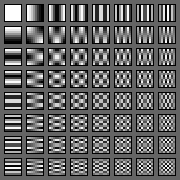
\includegraphics[width=0.4\textwidth]{./img/DCT_basis.png}
    \caption{Visualization of the DCT basis functions for an $8\times 8$ block.}
    \label{fig:dctbasis}
\end{figure}
This idea is shown in Figure~\ref{fig:dctbasis}, where the DCT basis functions for an $8\times 8$ block are visualized. The value of $DCT(i,j)$ represents the contribution of the corresponding basis function to the original block, and is calculated using the Equation~\ref{eq:dct_2D}, which is a two-dimensional extension of the DCT:
\begin{equation}
    DCT(i,j) = C(i)\cdot C(j)\cdot \dfrac{1}{\sqrt{2N}}\cdot \sum_{x=0}^{N-1}\sum_{y=0}^{N-1} f(x,y) \cos\left(\dfrac{(2x+1)\cdot i \pi}{2N}\right) \cos\left(\dfrac{(2y+1)\cdot j \pi}{2N}\right)
    \label{eq:dct_2D}
\end{equation}
where:
\begin{itemize}
    \item $N$ is the number of samples in each dimension of the original block (in this case, $8$).
    \item $f(x,y)$ is the value of the original block at position $(x,y)$ (the pixel value at that position).
    \item $C(i)$ and $C(j)$ are normalization factors defined as:
    \begin{equation*}
        C(t) = \begin{cases}
            \dfrac{1}{\sqrt{2}} & \text{if } t=0 \\[10pt]
            1 & \text{otherwise}
        \end{cases}
    \end{equation*}
\end{itemize}

This way, the original block is now represented in the frequency domain, where also $64$ coefficients are obtained but have different values and represent different aspects.

\subsubsection{Quantization of the DCT Coefficients}

In this step, a quantization matrix is used to reduce the precision of the DCT coefficients, which results in a loss of information but also in a significant reduction of the file size (as we will see). A matrix with the same dimension as the DCT coefficients (in this case, $8\times 8$) is used, where each element of the matrix represents the quantization step for the corresponding DCT coefficient.
\begin{itemize}
    \item Elements closer to the top-left corner of the matrix (lower frequencies) usually have smaller quantization steps (values in the matrix), as they represent important general information about the image that should not be lost.
    \item Elements closer to the bottom-right corner of the matrix (higher frequencies) usually have larger quantization steps, as they represent finer details in the image that can be more easily discarded without significantly affecting the perceived quality of the image. Therefore, bigger quantization steps are used to take those values to $0$.
\end{itemize}

This way, the $8\times 8$ block of DCT coefficients is transformed into a new $8\times 8$ block, where the value stored in the position $(i,j)$ is:
\begin{equation*}
    \ol{DCT}(i,j) = \text{round}\left(\dfrac{DCT(i,j)}{Q(i,j)}\right)
\end{equation*}
where $Q(i,j)$ is the quantization step for the coefficient at position $(i,j)$, and $\text{round}(\cdot)$ is the rounding function that rounds the result to the nearest integer.
This step is also lossy given two reasons:
\begin{itemize}
    \item The original DCT coefficients cannot be perfectly reconstructed from the quantized coefficients, as the quantization process involves rounding, which can lead to a loss of precision.
    \item The quantization process can lead to a significant loss of information where the quantized coefficients are taken to $0$, which can result in a significant loss of details in the image, especially in areas with high frequencies (fine details).
\end{itemize}

The election of the matrix $Q$ is crucial, as it can significantly affect the compression ratio and the perceived quality of the image. Some softwares allow the user to specify a quality factor, which in fact implies using different matrixes.

\subsubsection{Coefficient serialization}

Once the quantized DCT coefficients are obtained, they need to be serialized in order to be further compressed using Huffman encoding. This process is called ``dove tailing'' or ``zig-zag scanning'', because the coefficients are serialized in a zig-zag order, starting from the top-left corner of the block and moving towards the bottom-right corner. This way, the coefficients are ordered from lower frequencies to higher frequencies, which allows to take advantage of the fact that higher frequency coefficients are more likely to be zero after quantization, which can lead to better compression ratios when using Huffman encoding. The zig-zag order for an $8\times 8$ block is shown in Figure~\ref{fig:zigzag}.
\begin{figure}
    \centering
    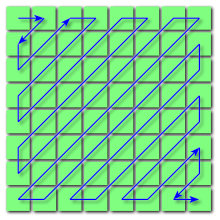
\includegraphics[width=0.4\textwidth]{./img/zigzag.png}
    \caption{Zig-zag order for an $8\times 8$ block.}
    \label{fig:zigzag}
\end{figure}



\subsubsection{Coefficient encoding}

After the coefficients are serialized, they need to be compressed. However, the DC coefficient is encoded differently than the AC coefficients.
\begin{description}
    \item[DC coefficient encoding]
    
    Given that the DC coefficient represents the average value of the block, it is likely to have similar values in adjacent blocks. Therefore, instead of encoding the DC coefficient directly, the difference between the DC coefficient of the current block and the DC coefficient of the previous block (the one to the left of the current block) is encoded. This way, if the DC coefficients of adjacent blocks are similar, the difference will be small.

    In order to encode the difference, two values are calculated:
    \begin{itemize}
        \item \ul{Size}: It is the number of bits that are required to represent the unsigned value of the difference. For instance, if the difference is $-5$, the size is $3$ because $5$ can be represented in $3$ bits as $101$.
        
        In order to encode the size, Huffman Encoding is used where smaller sizes have more probability that bigger sizes. A predifined Huffman tree is used.
        
        \item \ul{Amplitude}: It represents the actual value of the difference, and it is always represented using the number of bits specified by the size. For instance, if the difference is $-5$ and the size is $3$, the amplitude will have $3$ bits. The size $m$ represents values in the range $[-(2^{m}-1), 2^{m}-1]$, but the values in the range $[-(2^{m-1}-1), 2^{m-1}-1]$ belong to the previous size, so they are not include. Therefore, a mapping is performed: $-(2^{m}-1)$ is mapped to $0$, $-(2^{m}-1)+1$ is mapped to $1$, and so on. For instance, if the difference is $-5$ and the size is $3$, the amplitude will be $2$ because $-5$ is mapped to $2$ in the range of size $3$.
    \end{itemize}

    As stated, the size is encoded using Huffman encoding (which is deterministic given the prefix-free property), and therefore how many bits are used to encode the amplitude is determined by the size, so there is no need to encode the size of the amplitude separately.

    \item[AC coefficient encoding]
    
    The AC coefficients follow a different approach, as there may be many consecutive zero coefficients after quantization, especially for higher frequencies. Two symbols are used:
    \begin{itemize}
        \item \ul{Symbol 1}: It is a pair that represents:
        \begin{itemize}
            \item The number of consecutive zero coefficients before the current non-zero coefficient (using therefore RLE).
            \item The size of the current non-zero coefficient, which is calculated in the same way as the size of the DC coefficient difference.
        \end{itemize}
        This pair is encoded using Huffman encoding using some predefined tables. Two important pairs should be noted:
        \begin{itemize}
            \item $(0,0)$: It represents the end of the block, and it is used when all the remaining coefficients in the block are zero. It can also be written as \texttt{EOB} (End Of Block).
            \item $(15,0)$: It represents a run of $16$ consecutive zero coefficients, and it is used when there are more than $15$ consecutive zero coefficients before a non-zero coefficient. It can also be written as \texttt{ZRL} (Zero Run Length).
        \end{itemize}
        \item \ul{Symbol 2}: It represents the actual value of the current non-zero coefficient, and it is encoded in the same way as the amplitude of the DC coefficient difference, using the size of the current non-zero coefficient to determine how many bits are used to encode the value.
    \end{itemize}

    The encoding of the AC coefficients is done by first encoding the symbol 1 using Huffman encoding, and then encoding the symbol 2 using the size of the current non-zero coefficient to determine how many bits are used to encode the value.
\end{description}